% Chapter 6 — GPU Architecture, CUDA Programming, and Maximizing Occupancy
% Style follows chapter01/02 presentations (LaTeX Beamer, Madrid, navy).
% Compile: pdflatex chapter06-presentation.tex  (run twice)
\documentclass[aspectratio=169]{beamer}

% ====== Presenter info: EDIT ME ======
\newcommand{\PresenterName}{Your Name}          % <-- 改成你的名字
\newcommand{\PresenterTitle}{Applied Scientist} % <-- 改成你的头衔
\newcommand{\PresenterOrg}{AWS}
% =====================================

\usetheme{Madrid}
\definecolor{navy}{RGB}{18,47,90}
\definecolor{kwblue}{RGB}{0,56,132}
\definecolor{okgreen}{RGB}{80,130,20}
\usecolortheme[named=navy]{structure}
\setbeamercolor{frametitle}{bg=navy,fg=white}
\setbeamercolor{title}{bg=navy,fg=white}
\setbeamercolor{block title}{bg=navy,fg=white}
\setbeamercolor{block body}{bg=gray!12,fg=black}
\setbeamercolor{block title example}{bg=okgreen,fg=white}
\setbeamercolor{block body example}{bg=okgreen!10,fg=black}
\setbeamertemplate{navigation symbols}{}
\setbeamertemplate{blocks}[rounded][shadow=true]

\usepackage{booktabs}
\usepackage{listings}
\lstset{
  language=C++,
  basicstyle=\ttfamily\fontsize{6.5}{7.6}\selectfont,
  keywordstyle=\color{kwblue}\bfseries,
  commentstyle=\color{gray}\itshape,
  stringstyle=\color{okgreen},
  showstringspaces=false,
  breaklines=true,
  columns=fullflexible
}

\newcommand{\kw}[1]{\textbf{\textcolor{kwblue}{#1}}}
\newcommand{\pe}[1]{{\footnotesize\itshape Plain English: #1}}
\newcommand{\refmark}[1]{\textsuperscript{[#1]}}

\title[AI Systems Performance Engineering]{AI Systems Performance Engineering}
\subtitle{Chapter 6 --- GPU Architecture, CUDA Programming, and Maximizing Occupancy}
\author[\PresenterName\ \ \PresenterTitle\ \ \PresenterOrg]{\PresenterName\\\PresenterTitle\\\PresenterOrg}
\institute[]{\footnotesize Internal Training for Applied Scientists on AI Infrastructure}
\date{August 15, 2026}

\begin{document}

% ---------------------------------------------------------------- 1
\begin{frame}
  \titlepage
\end{frame}

% ---------------------------------------------------------------- 2
\begin{frame}{What This Talk Is About --- and Why}
  \begin{block}{In plain English}
    A GPU is a \kw{throughput machine}: it runs \kw{thousands of threads} at once and hides slow memory by
    always having other work ready. This chapter teaches the \kw{vocabulary} (warps, blocks, grids, SMs),
    the \kw{memory ladder} (registers $\to$ shared $\to$ L2 $\to$ HBM), and the \kw{one golden rule}:
    launch enough parallel work to keep every SM busy.
  \end{block}
  \begin{columns}[t]
    \column{0.48\textwidth}
    \begin{itemize}
      \item \kw{The problem:} a GPU with idle SMs is an expensive space heater --- most naive kernels
            use a few percent of the hardware.
      \item \kw{The tool:} CUDA's thread hierarchy maps your algorithm onto hardware, unchanged across GPU generations.
    \end{itemize}
    \column{0.48\textwidth}
    \begin{itemize}
      \item \kw{The metric:} \emph{occupancy} --- how many warps are in flight vs.\ the hardware maximum.
      \item \kw{The compass:} the \emph{roofline model} tells you if a kernel is compute-bound or memory-bound
            before you optimize the wrong thing.
    \end{itemize}
  \end{columns}
  \medskip
  \centering\footnotesize\itshape
  This is the foundation chapter for everything kernel-level in Chapters 7--12.
\end{frame}

% ---------------------------------------------------------------- 3
\begin{frame}{Roadmap}
  \begin{enumerate}
    \item \kw{GPU architecture} --- SMs, warp schedulers, threads/blocks/grids, warp divergence
    \item \kw{CUDA programming refresher} --- kernel anatomy, launch parameters, async allocation
    \item \kw{Memory hierarchy} --- registers, shared/L1, TMEM, L2, HBM3e, Unified Memory
    \item \kw{Occupancy} --- why parallelism is rule \#1; a 22$\times$ case study; launch bounds
    \item \kw{Correctness} --- NVIDIA Compute Sanitizer
    \item \kw{Roofline model} --- compute-bound vs.\ memory-bound, and what to do about each
  \end{enumerate}
  \medskip
  \pe{first make the GPU busy, then make each cycle count, and always profile to know which fix applies.}
\end{frame}

% ---------------------------------------------------------------- 4
\begin{frame}{GPUs Optimize Throughput; CPUs Optimize Latency}
  \begin{columns}[c]
    \column{0.55\textwidth}
    \begin{itemize}
      \item CPUs: few cores, deep caches, fast \emph{single} threads. GPUs: hundreds of \kw{SMs}
            (streaming multiprocessors) running \kw{thousands of threads} in parallel.
      \item Basic CUDA flow: host copies data \kw{CPU $\to$ GPU}, launches a \kw{kernel},
            copies results back.
      \item The GPU hides transfer and memory latency with \kw{massive parallelism}:
            when one warp waits, another runs.
      \item Each Blackwell SM tracks up to \kw{64 warps} (2{,}048 threads) concurrently.\refmark{1,2}
    \end{itemize}
    \column{0.42\textwidth}
    \centering
    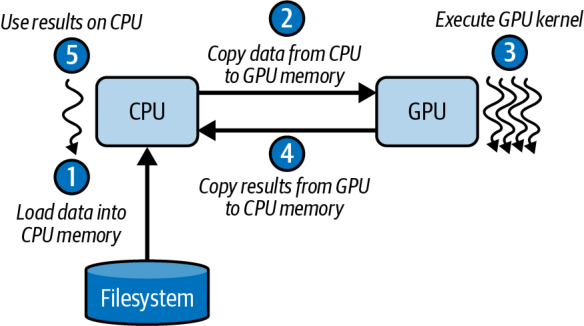
\includegraphics[width=\linewidth]{figs/fig6-1.png}\\
    {\scriptsize Figure 6-1. Simple CUDA programming flow}
  \end{columns}
  \medskip
  \pe{the CPU is a sports car, the GPU is a freight train --- don't ask the train to be fast, ask it to be \emph{full}.}
\end{frame}

% ---------------------------------------------------------------- 5
\begin{frame}{Inside a Blackwell SM: Four Schedulers, Dual Issue}
  \begin{columns}[c]
    \column{0.52\textwidth}
    \begin{itemize}
      \item Each SM = four ``\kw{mini-SMs}'': independent warp schedulers sharing on-chip resources.
      \item Each scheduler issues \kw{1 warp instruction/cycle}, and can \kw{dual-issue}
            one math + one memory op \emph{from the same warp}.
      \item Best case: \kw{4 math + 4 memory} instructions per cycle across 4 warps.
      \item \kw{SFUs} (sin, cos, sqrt, \ldots) run in a separate pipeline --- transcendentals don't stall the core pipes.
      \item Per SM: \kw{64K 32-bit registers} (256 KB), \kw{256 KB} unified L1/shared memory.\refmark{2}
    \end{itemize}
    \column{0.45\textwidth}
    \centering
    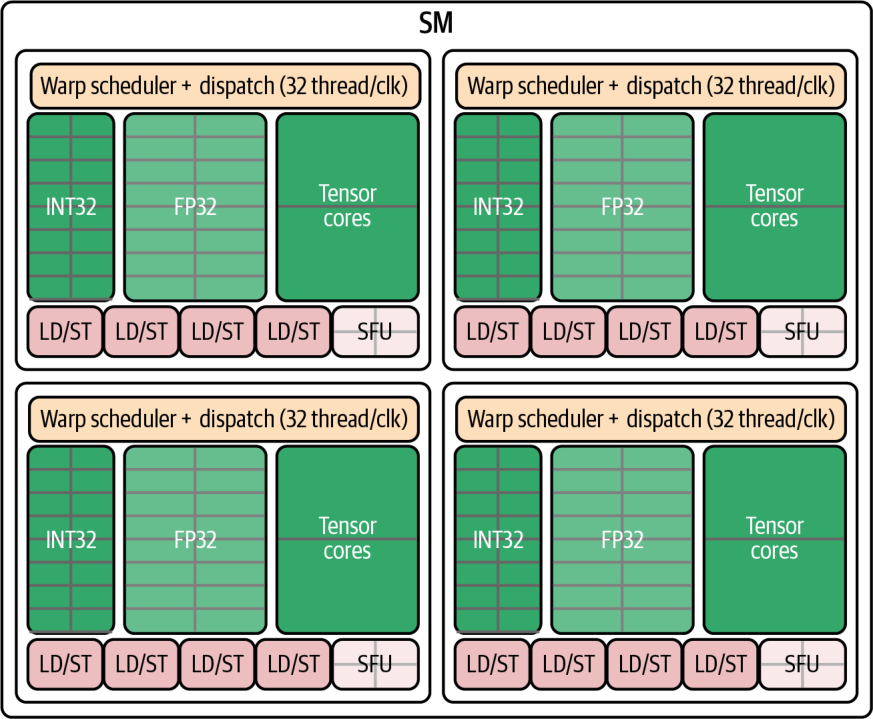
\includegraphics[width=0.82\linewidth]{figs/fig6-2.png}\\
    {\scriptsize Figure 6-2. Four warp schedulers with dual issue (math + memory)}
  \end{columns}
  \medskip
  \pe{four checkout lanes; each cashier scans with one hand and bags with the other.}
\end{frame}

% ---------------------------------------------------------------- 6
\begin{frame}{The Thread Hierarchy: Threads $\to$ Blocks $\to$ Grids}
  \begin{columns}[c]
    \column{0.52\textwidth}
    \begin{itemize}
      \item \kw{Thread}: runs your kernel code on one data element.
      \item \kw{Thread block} (CTA): up to \kw{1{,}024 threads}; shares fast \kw{shared memory};
            synchronizes with \texttt{\_\_syncthreads()} (minimize barriers --- they cost time).
      \item \kw{Grid}: all blocks of one launch; scales to \kw{millions of threads} with no kernel changes.
      \item Blocks execute \kw{independently, in any order} --- that freedom is what lets the same code
            run on future GPUs with more SMs.
    \end{itemize}
    \column{0.45\textwidth}
    \centering
    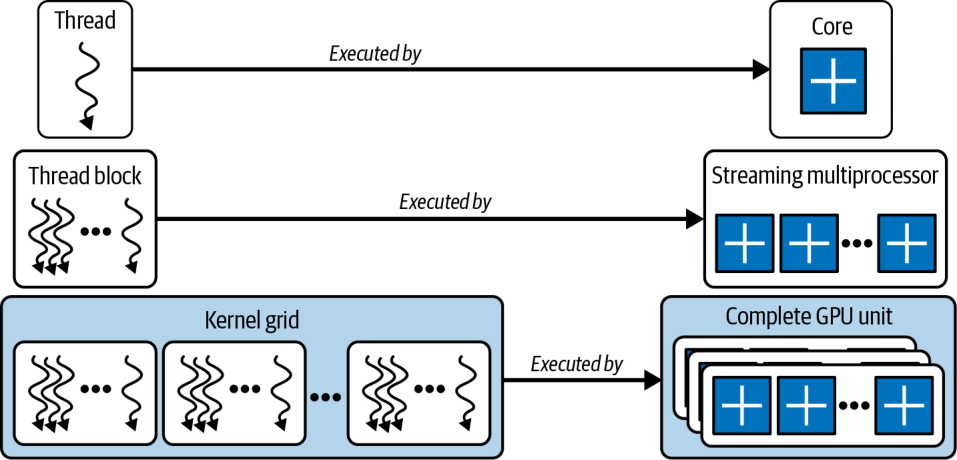
\includegraphics[width=\linewidth]{figs/fig6-3.png}\\
    {\scriptsize Figure 6-3. Threads, thread blocks (CTAs), and grids}
  \end{columns}
  \medskip
  \pe{workers (threads) form teams (blocks) that can talk cheaply inside the team; the company (grid) hires as many teams as the job needs.}
\end{frame}

% ---------------------------------------------------------------- 7
\begin{frame}{Warps and SIMT: 32 Threads in Lockstep}
  \begin{columns}[c]
    \column{0.52\textwidth}
    \begin{itemize}
      \item Blocks are subdivided into \kw{warps of 32 threads} that execute one instruction together
            (\kw{SIMT}: single instruction, multiple threads).
      \item \kw{Occupancy} = fraction of an SM's warp slots that are occupied by active warps.
            High occupancy $\Rightarrow$ when one warp stalls on memory, another is ready $\Rightarrow$
            \kw{latency hiding}.
      \item Balance against per-thread resources: too many registers/shared memory per thread
            $\Rightarrow$ fewer resident warps, or \kw{register spilling} to slow memory.
    \end{itemize}
    \column{0.45\textwidth}
    \centering
    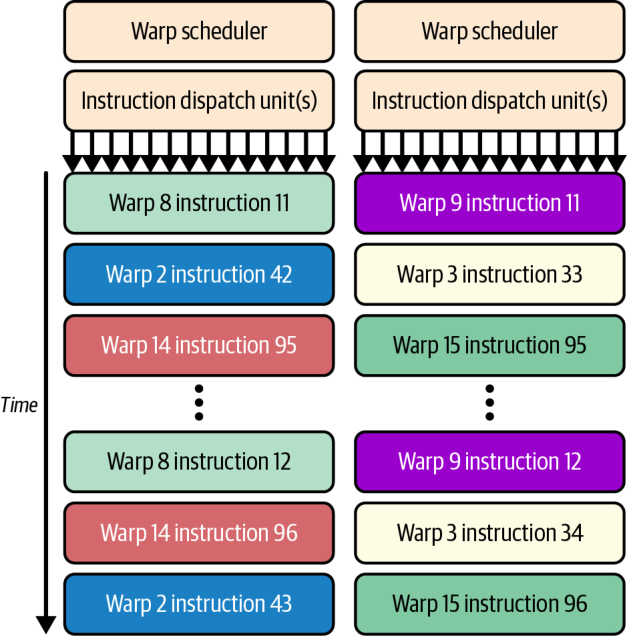
\includegraphics[width=0.8\linewidth]{figs/fig6-7.png}\\
    {\scriptsize Figure 6-7. A warp advances as a whole under the warp scheduler}
  \end{columns}
  \medskip
  \pe{a warp is a rowing crew of 32 --- everyone pulls the same stroke at the same time, or the boat waits.}
\end{frame}

% ---------------------------------------------------------------- 8
\begin{frame}{Warp Divergence: When {\ttfamily if/else} Splits the Crew}
  \begin{columns}[c]
    \column{0.52\textwidth}
    \begin{itemize}
      \item If threads \emph{within one warp} take different branches, the warp \kw{serializes}:
            it runs the \texttt{if} path with half the lanes masked, then the \texttt{else} path.
      \item Execution time multiplies by the \kw{number of distinct paths}.
      \item \kw{No penalty across warps} --- different warps may branch differently for free.
      \item Detection and mitigation: Chapter 8 (profile with Nsight Compute).
    \end{itemize}
    \column{0.45\textwidth}
    \centering
    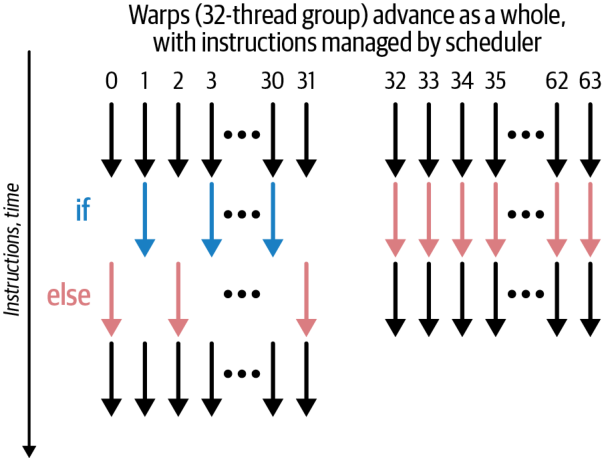
\includegraphics[width=0.85\linewidth]{figs/fig6-8.png}\\
    {\scriptsize Figure 6-8. SIMT warp divergence (left) vs.\ uniformity (right)}
  \end{columns}
  \medskip
  \pe{if half the rowing crew rows left and half rows right, the boat does each maneuver twice --- slowly.}
\end{frame}

% ---------------------------------------------------------------- 9
\begin{frame}{Hardware Limits That Shape Your Launch (Blackwell B200)}
  \begin{columns}[c]
    \column{0.55\textwidth}
    {\small
    \begin{tabular}{@{}ll@{}}
      \toprule
      \textbf{Resource} & \textbf{Limit} \\
      \midrule
      Warp size & 32 threads \\
      Max threads / block & 1{,}024 \ (= 32 warps) \\
      Max resident warps / SM & \kw{64} \ (2{,}048 threads) \\
      Max resident blocks / SM & 32 \\
      Registers / SM & 64K $\times$ 32-bit (255 / thread) \\
      Shared memory / SM & 228 KB (227 usable) \\
      Max grid (X dim) & 2{,}147{,}483{,}647 blocks \\
      Max concurrent grids & 128 \\
      \bottomrule
    \end{tabular}}
    \column{0.42\textwidth}
    \centering
    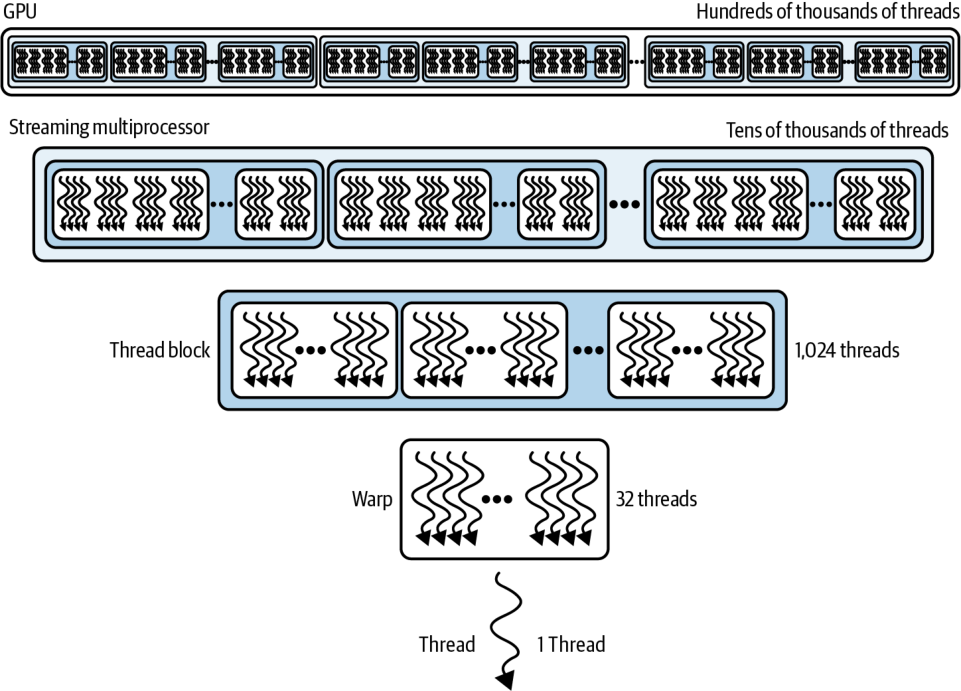
\includegraphics[width=\linewidth]{figs/fig6-9.png}\\
    {\scriptsize Figure 6-9. Relative scale of thread resources}
  \end{columns}
  \smallskip
  \begin{itemize}\small
    \item Pick block sizes that are \kw{multiples of 32} --- a 33-thread block burns two warp slots,
          one of them 31/32 empty. You hit \kw{per-SM limits} long before grid limits.\refmark{1,2}
  \end{itemize}
\end{frame}

% ---------------------------------------------------------------- 10
\begin{frame}[fragile]{Anatomy of a CUDA Kernel}
  \begin{columns}[t]
    \column{0.55\textwidth}
\begin{lstlisting}
__global__ void myKernel(float* input, int N) {
    // unique global index for this thread
    int idx = blockIdx.x * blockDim.x + threadIdx.x;
    if (idx < N) {            // bounds check!
        input[idx] *= 2.0f;
    }
}
// host side:
const int threadsPerBlock = 256;               // 8 warps
const int blocksPerGrid =
    (N + threadsPerBlock - 1) / threadsPerBlock; // round up
myKernel<<<blocksPerGrid, threadsPerBlock>>>(d_input, N);
cudaDeviceSynchronize();
\end{lstlisting}
    \column{0.42\textwidth}
    \begin{itemize}\small
      \item \kw{\texttt{\_\_global\_\_}} marks device code; \kw{\texttt{<<<blocks, threads>>>}}
            configures the launch.
      \item The kernel is written for \kw{one thread}; \texttt{idx} carves out its slice of the data.
      \item The \kw{bounds check} \texttt{if (idx < N)} protects the last, partially-filled block
            from illegal memory accesses.
      \item Errors surface \kw{lazily} --- check \texttt{cudaGetLastError()} after launches.
    \end{itemize}
  \end{columns}
  \smallskip
  \pe{write the job for \emph{one} worker; CUDA prints a million copies, each with a different row number.}
\end{frame}

% ---------------------------------------------------------------- 11
\begin{frame}{Choosing Launch Parameters}
  \begin{block}{Recipe that works almost everywhere}
    Start with \kw{\texttt{threadsPerBlock = 256}} (8 warps);
    \kw{\texttt{blocksPerGrid = (N + 255) / 256}} to cover every element. Then tune (128/512) by profiling.
  \end{block}
  \begin{itemize}
    \item \kw{Multiple of 32}: no half-empty warps occupying scheduler slots.
    \item \kw{Latency hiding}: hundreds of threads per SM keep pipelines busy during DRAM stalls.
    \item \kw{Resource balance}: 256 rarely exhausts registers or shared memory; 256--512 is the
          sweet spot on Blackwell.
    \item 2D/3D data: same pattern with \texttt{dim3} --- e.g., $16\times16$ blocks over a
          $1{,}024\times1{,}024$ image, with a 2D bounds check.
  \end{itemize}
  \medskip
  \pe{256 is the ``medium coffee'' of block sizes --- almost never the wrong first order, refine later if profiling says so.}
\end{frame}

% ---------------------------------------------------------------- 12
\begin{frame}[fragile]{Allocate Asynchronously: Streams and Memory Pools}
  \begin{columns}[t]
    \column{0.52\textwidth}
\begin{lstlisting}
cudaStream_t s;
cudaStreamCreateWithFlags(&s, cudaStreamNonBlocking);

float* d_buf = nullptr;
cudaMallocAsync(&d_buf, N * sizeof(float), s);
myKernel<<<blocks, threads, 0, s>>>(d_buf, N);
cudaFreeAsync(d_buf, s);  // deferred until s finishes
\end{lstlisting}
    \begin{itemize}
      \item Tune the pool: \texttt{cudaMemPoolAttrReleaseThreshold},
            \texttt{cudaMemPoolTrimTo}.
    \end{itemize}
    \column{0.45\textwidth}
    \begin{itemize}\small
      \item \texttt{cudaMalloc}/\texttt{cudaFree} are \kw{synchronous and expensive}:
            full-device sync + OS calls (\texttt{mmap}/\texttt{ioctl}).
      \item \kw{\texttt{cudaMallocAsync}/\texttt{cudaFreeAsync}} draw from a per-device
            \kw{memory pool}: recycled buffers, no global sync, less fragmentation.
      \item \kw{PyTorch's caching allocator} (\texttt{PYTORCH\_ALLOC\_CONF}) does the same trick for tensors.
      \item Non-blocking streams avoid legacy \kw{default-stream barriers}.
    \end{itemize}
  \end{columns}
  \smallskip
  \pe{keep a truck fleet in the lot and grab keys --- don't buy and return a truck for every delivery.}
\end{frame}

% ---------------------------------------------------------------- 13
\begin{frame}{The GPU Memory Hierarchy (Blackwell)}
  \begin{columns}[c]
    \column{0.58\textwidth}
    {\scriptsize\setlength{\tabcolsep}{3.5pt}
    \begin{tabular}{@{}lllll@{}}
      \toprule
      \textbf{Level} & \textbf{Scope} & \textbf{Capacity} & \textbf{Latency} & \textbf{BW} \\
      \midrule
      Registers & thread & 256 KB / SM & $\sim$1 cyc & 10s TB/s \\
      Shared + L1 & SM & 228 KB usable & 20--30 cyc & TB/s \\
      TMEM & SM & 256 KB (TC) & $\sim$10 cyc & TB/s \\
      Const cache & SM & 8 of 64 KB & 1 cyc bcast & TB/s \\
      L2 cache & GPU & \kw{126 MB} & $\sim$200 cyc & multi-TB/s \\
      Local (spill) & thread & DRAM-backed & $\leq$1000 cyc & --- \\
      Global HBM3e & device & \kw{180 GB} (B200) & $\leq$1000 cyc & \kw{$\sim$8 TB/s} \\
      \bottomrule
    \end{tabular}}
    \medskip
    \begin{itemize}\small
      \item Rule: \kw{maximize reuse} in registers/shared/L2; touch HBM as rarely
            --- and as \kw{coalesced} (128-byte aligned) --- as possible.
    \end{itemize}
    \column{0.39\textwidth}
    \centering
    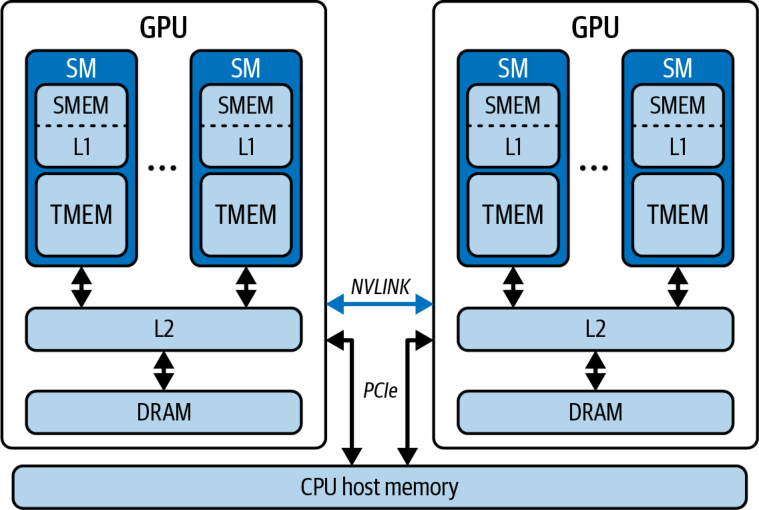
\includegraphics[width=\linewidth]{figs/fig6-10.png}\\
    {\scriptsize Figure 6-10. GPU memory hierarchy, including the CPU}
  \end{columns}
  \medskip
  \pe{desk (registers) $\to$ office shelf (shared) $\to$ building library (L2) $\to$ warehouse across town (HBM). Do your work at the desk.}
\end{frame}

% ---------------------------------------------------------------- 14
\begin{frame}{TMEM and TMA: Feeding the Tensor Cores}
  \begin{columns}[c]
    \column{0.55\textwidth}
    \begin{itemize}
      \item \kw{TMEM}: dedicated \kw{256 KB per-SM SRAM} that acts as the \kw{accumulator}
            for 5th-gen Tensor Core ops (\texttt{tcgen05.*}, UMMA); tens of TB/s to the Tensor Cores.
      \item Not pointer-addressable from CUDA C++ --- data movement is orchestrated by the
            \kw{TMA} (Tensor Memory Accelerator) via descriptors: global $\leftrightarrow$ SMEM
            $\leftrightarrow$ TMEM.
      \item For $C = A \times B$: operand B in SMEM, A + accumulator in TMEM;
            tiles flow from HBM through L2 by TMA.
      \item Details in Chapter 10 --- here, know that it exists and \kw{reduces global-memory pressure}.
    \end{itemize}
    \column{0.42\textwidth}
    \centering
    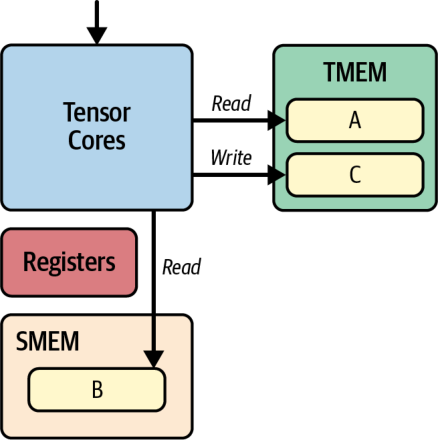
\includegraphics[width=0.75\linewidth]{figs/fig6-11.png}\\
    {\scriptsize Figure 6-11. TMEM + SMEM servicing Tensor Cores for $C = A\times B$}
  \end{columns}
  \medskip
  \pe{TMA is a forklift crew moving pallets in the background; the chefs never leave the kitchen.}
\end{frame}

% ---------------------------------------------------------------- 15
\begin{frame}[fragile]{Unified Memory: One Address Space, Hidden Migrations}
  \begin{columns}[c]
    \column{0.55\textwidth}
    \begin{itemize}
      \item \kw{\texttt{cudaMallocManaged()}}: one coherent CPU+GPU address space; pages
            \kw{migrate on demand} --- no manual \texttt{cudaMemcpy}.
      \item Cost: a GPU touch of a CPU-resident page \kw{page-faults and stalls} the kernel.
      \item On Grace superchips, \kw{NVLink-C2C} ($\sim$900 GB/s) makes migrations far cheaper
            than PCIe --- but never free.
      \item Fix ``surprise'' stalls proactively:
    \end{itemize}
\begin{lstlisting}
cudaMemPrefetchAsync(ptr, size, gpuId, s); // move it BEFORE launch
cudaMemAdvise(ptr, size, cudaMemAdviseSetPreferredLocation, gpuId);
cudaMemAdvise(ptr, size, cudaMemAdviseSetReadMostly, gpuId);
cudaStreamAttachMemAsync(stream, ptr, 0, cudaMemAttachSingle);
\end{lstlisting}
    \column{0.42\textwidth}
    \centering
    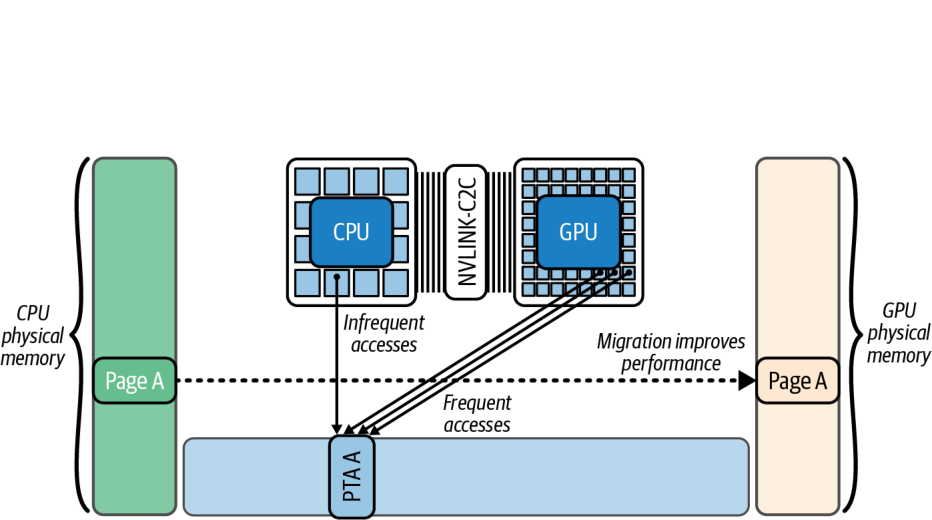
\includegraphics[width=\linewidth]{figs/fig6-16.png}\\
    {\scriptsize Figure 6-16. Automatic page migration with Unified Memory}
  \end{columns}
  \medskip
  \pe{Unified Memory is room service: convenient, but if you don't order ahead (prefetch), you wait hungry at kernel time.}
\end{frame}

% ---------------------------------------------------------------- 16
\begin{frame}[fragile]{Occupancy Case Study: One Thread vs.\ Many}
  \begin{columns}[t]
    \column{0.5\textwidth}
    {\small\kw{Sequential} --- one thread does everything:}
\begin{lstlisting}
__global__ void addSequential(const float* A,
    const float* B, float* C, int N) {
  if (blockIdx.x == 0 && threadIdx.x == 0)
    for (int i = 0; i < N; ++i)
      C[i] = A[i] + B[i];
}
addSequential<<<1,1>>>(dA, dB, dC, N);
\end{lstlisting}
    {\small Same trap in PyTorch: a Python \texttt{for} loop of \texttt{C[i] = A[i] + B[i]} launches
    \kw{N tiny serial kernels}.}
    \column{0.47\textwidth}
    {\small\kw{Parallel} --- one thread per element:}
\begin{lstlisting}
__global__ void addParallel(const float* A,
    const float* B, float* C, int N) {
  int idx = blockIdx.x*blockDim.x + threadIdx.x;
  if (idx < N) C[idx] = A[idx] + B[idx];
}
addParallel<<<(N+255)/256, 256>>>(dA, dB, dC, N);
\end{lstlisting}
    {\small PyTorch equivalent: just \kw{\texttt{C = A + B}} --- one vectorized kernel.}
  \end{columns}
  \medskip
  \pe{the most common GPU performance bug is not a slow kernel --- it's accidentally using the GPU as a very expensive single-core CPU.}
\end{frame}

% ---------------------------------------------------------------- 17
\begin{frame}{Case Study Results: 22$\times$ from Occupancy Alone}
  \begin{columns}[c]
    \column{0.52\textwidth}
    {\small
    \begin{tabular}{@{}lrr@{}}
      \toprule
      \textbf{Metric} & \textbf{Sequential} & \textbf{Parallel} \\
      \midrule
      Kernel time (ms) & 48.21 & \kw{2.17} \\
      GPU utilization & 1.5\% & \kw{95\%} \\
      Achieved occupancy & 1.3\% & \kw{38.7\%} \\
      Warp exec.\ efficiency & 3.1\% & \kw{100\%} \\
      \bottomrule
    \end{tabular}}\\[4pt]
    {\scriptsize Table 6-6 (illustrative numbers --- see the book's GitHub repo\refmark{7} for real benchmarks)}
    \column{0.45\textwidth}
    \centering
    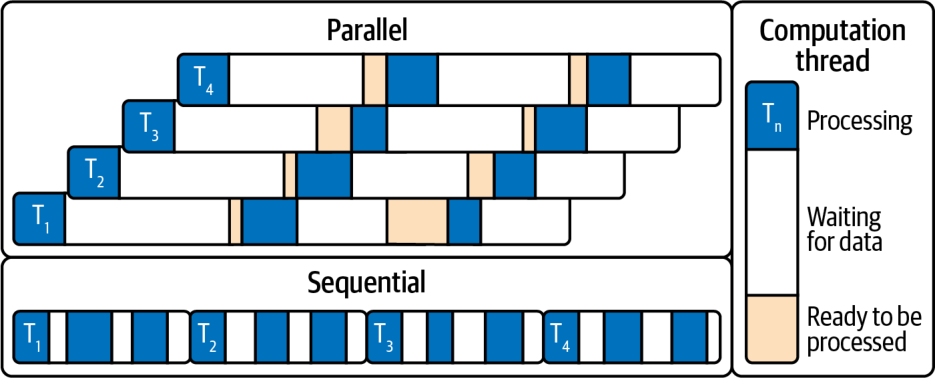
\includegraphics[width=\linewidth]{figs/fig6-20.png}\\
    {\scriptsize Figure 6-20. Sequential timeline has idle gaps; parallel fills them with other warps' work}
  \end{columns}
  \medskip
  \begin{itemize}
    \item Rule \#1 of CUDA performance: \kw{launch enough parallel work}. Aim for occupancy
          in the \kw{80--100\%} range \emph{if} performance is poor and occupancy is low.
    \item But: at high occupancy with a \kw{memory-bound} kernel, more warps won't help ---
          the bottleneck is bandwidth (see roofline).
  \end{itemize}
\end{frame}

% ---------------------------------------------------------------- 18
\begin{frame}[fragile]{Tuning Occupancy: Launch Bounds and the Occupancy API}
  \begin{columns}[t]
    \column{0.52\textwidth}
\begin{lstlisting}
// promise <=256 threads/block; ask for >=16 blocks/SM
__global__ __launch_bounds__(256, 16)
void myKernel(...) { /* ... */ }

// autotune block size at runtime:
int minGridSize = 0, bestBlockSize = 0;
cudaOccupancyMaxPotentialBlockSize(
    &minGridSize, &bestBlockSize, myKernel,
    dynSmemBytes, /*blockSizeLimit=*/0);
int gridSize = std::max(minGridSize,
    (N + bestBlockSize - 1) / bestBlockSize);
\end{lstlisting}
    \column{0.45\textwidth}
    \begin{itemize}
      \item \kw{\texttt{\_\_launch\_bounds\_\_}} lets the compiler cap registers/inlining so
            \kw{more warps fit per SM} (hardware clamps impossible requests, e.g.\ 16$\times$256 $>$ 2{,}048).
      \item \kw{Trade-off}: fewer registers per thread $\Rightarrow$ more resident warps,
            but too few $\Rightarrow$ \kw{spilling to local memory} (slow!).
      \item \kw{Validate} API suggestions by timing $\pm$1--2 block-size candidates ---
            slightly sub-maximal occupancy is sometimes faster.
    \end{itemize}
  \end{columns}
  \medskip
  \pe{you're trading each worker's toolbox size for the number of workers on the floor --- the sweet spot is empirical.}
\end{frame}

% ---------------------------------------------------------------- 19
\begin{frame}{Debugging Correctness: NVIDIA Compute Sanitizer}
  \begin{columns}[t]
    \column{0.48\textwidth}
    \begin{block}{Memory}
      \begin{itemize}\small
        \item \kw{memcheck} --- out-of-bounds / misaligned accesses, device leaks.
        \item \kw{initcheck} --- reads of uninitialized global memory (missing H2D copy?).
      \end{itemize}
    \end{block}
    \column{0.48\textwidth}
    \begin{exampleblock}{Concurrency}
      \begin{itemize}\small
        \item \kw{racecheck} --- shared-memory hazards (WAW / WAR / RAW).
        \item \kw{synccheck} --- invalid barriers, deadlock-causing sync.
      \end{itemize}
    \end{exampleblock}
  \end{columns}
  \medskip
  \begin{itemize}
    \item CLI: \texttt{compute-sanitizer [--tool <name>] <app>}; filter with
          \texttt{--kernel-name}, annotate with \kw{NVTX}.
    \item Put it in \kw{CI} with \texttt{--error-exitcode} --- catch correctness regressions before they ship.\refmark{5}
  \end{itemize}
  \medskip
  \pe{with 100{,}000 threads, ``it works on my run'' means nothing --- the sanitizer is your seatbelt for race conditions you'll never reproduce by hand.}
\end{frame}

% ---------------------------------------------------------------- 20
\begin{frame}{The Roofline Model: Which Wall Are You Hitting?}
  \begin{columns}[c]
    \column{0.5\textwidth}
    \begin{itemize}
      \item \kw{Arithmetic intensity} = FLOPs per byte moved to/from HBM.
      \item Two ceilings: \kw{flat} compute roof ($\sim$80 TFLOP/s FP32) and \kw{sloped}
            memory roof ($\sim$8 TB/s). They cross at the \kw{ridge point} $\approx$ 10 FLOPs/byte.
      \item Example: \texttt{C = A + B} does 1 FLOP per 12 bytes $\Rightarrow$
            \kw{0.083 FLOPs/byte} --- $>$100$\times$ left of the ridge: hopelessly \kw{memory-bound}.
      \item LLMs: \kw{prefill} tends compute-bound; \kw{decode} (streaming weights) is memory-bound.
    \end{itemize}
    \column{0.47\textwidth}
    \centering
    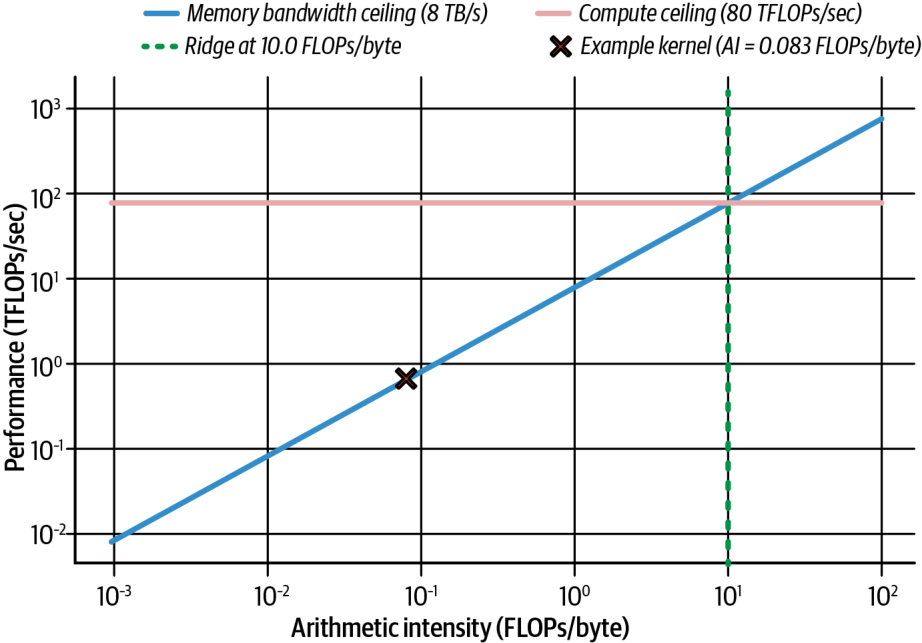
\includegraphics[width=\linewidth]{figs/fig6-21.png}\\
    {\scriptsize Figure 6-21. Roofline for a Blackwell-class GPU with our kernel at 0.083 FLOPs/byte}
  \end{columns}
  \medskip
  \pe{the roofline asks first: is this kernel starving for math, or for data?}\refmark{4}
\end{frame}

% ---------------------------------------------------------------- 21
\begin{frame}{Moving Right on the Roofline: Lower Precision Pays Twice}
  \begin{itemize}
    \item To escape the memory-bound region, \kw{do more work per byte}: reuse data on-chip,
          fuse ops --- or simply \kw{shrink the bytes}.
    \item One 128-byte transaction carries \kw{32 FP32 = 64 FP16 = 128 FP8 = 256 FP4} values.
          FP32 $\to$ FP16 instantly \kw{doubles} FLOPs/byte.
    \item Blackwell adds \kw{FP8 and FP4 Tensor Cores}, plus \kw{hardware decompression}:
          weights stored compressed in HBM are expanded on the fly --- effectively more bandwidth.
    \item That's why Blackwell shines on memory-bound \kw{token generation}: 4-bit weights
          in HBM, decompressed and upcast for accumulation.
  \end{itemize}
  \medskip
  \begin{block}{The takeaway}
    Precision is a \kw{bandwidth} optimization as much as a compute one:
    halve the bytes $\Rightarrow$ double the arithmetic intensity $\Rightarrow$ move toward the compute roof.
  \end{block}
\end{frame}

% ---------------------------------------------------------------- 22
\begin{frame}{Profiling Workflow: nsys for \emph{When}, ncu for \emph{Why}}
  \begin{columns}[c]
    \column{0.52\textwidth}
    \begin{itemize}
      \item \kw{Nsight Systems} (\texttt{nsys}): whole-app timeline --- GPU idle gaps, CPU overlap,
            PCIe/NVLink transfers. \pe{a stopwatch for the whole machine.}
      \item \kw{Nsight Compute} (\texttt{ncu}): per-kernel counters --- occupancy, stall reasons,
            cache hit rates, DRAM utilization. \pe{a microscope on one kernel.}
      \item Wrap suspect regions in \kw{NVTX} ranges to see them on the timeline.
      \item Memory-bound signature: \kw{high DRAM utilization + low ALU utilization};
            missing async overlap often = \kw{no pinned memory} or default-stream sync.
    \end{itemize}
    \column{0.45\textwidth}
    \centering
    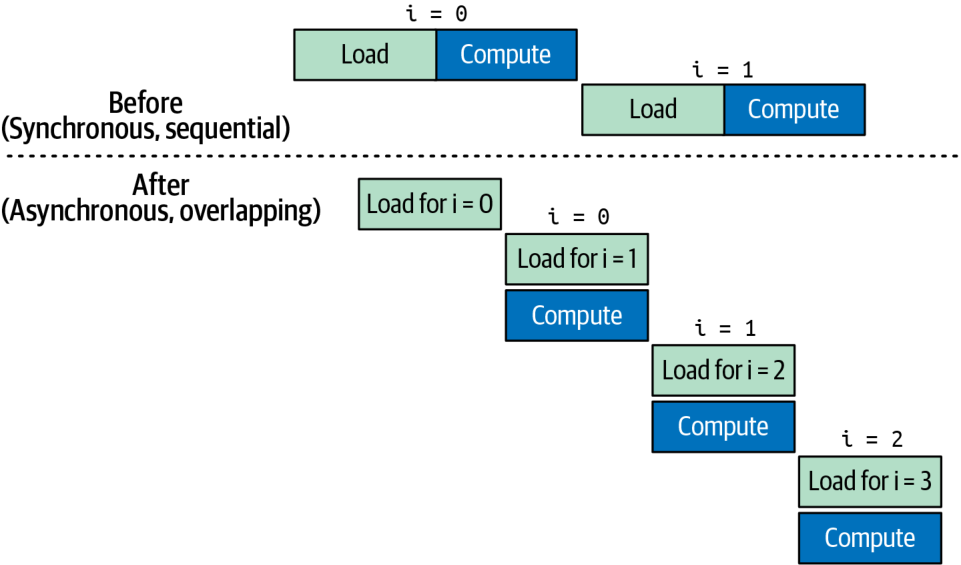
\includegraphics[width=\linewidth]{figs/fig6-22.png}\\
    {\scriptsize Figure 6-22. Sync (sequential) vs.\ async (overlapped) transfers + compute}
  \end{columns}
\end{frame}

% ---------------------------------------------------------------- 23
\begin{frame}{Key Takeaways}
  \begin{columns}[t]
    \column{0.48\textwidth}
    \begin{itemize}\small
      \item \kw{SIMT}: 32-thread warps in lockstep; keep many warps in flight to hide latency.
      \item \kw{Hierarchy}: threads $\to$ blocks ($\leq$1{,}024) $\to$ grids; blocks independent
            $\Rightarrow$ portable scaling.
      \item \kw{Block size}: multiples of 32; start at 256; respect per-SM limits
            (64 warps, 32 blocks, 228 KB shared, 255 regs/thread).
      \item \kw{Async allocation}: \texttt{cudaMallocAsync} + streams + pools;
            PyTorch's caching allocator does this for you.
    \end{itemize}
    \column{0.48\textwidth}
    \begin{itemize}\small
      \item \kw{Memory ladder}: registers $\to$ shared/L1 $\to$ L2 $\to$ HBM;
            reuse up high, coalesce down low.
      \item \kw{Unified Memory}: convenient, but prefetch + advise to avoid page-fault stalls.
      \item \kw{Roofline}: FLOPs/byte decides memory- vs.\ compute-bound;
            lower precision moves you right.
      \item \kw{Occupancy is necessary, not sufficient}: high occupancy can't fix a
            bandwidth-limited kernel --- profile, then optimize.
    \end{itemize}
  \end{columns}
\end{frame}

% ---------------------------------------------------------------- 24
\begin{frame}{Conclusion and What's Next}
  \begin{block}{This chapter in one sentence}
    Make the GPU \kw{busy} (occupancy), make data \kw{close} (memory hierarchy),
    and let the \kw{roofline} tell you which battle to fight next.
  \end{block}
  \begin{itemize}
    \item Max occupancy is \kw{not always optimal}: enough ILP per thread can beat more warps;
          sometimes fewer threads with more registers each wins. \kw{Benchmark it.}
    \item Coming next in the book: warp divergence and memory-access tuning (Ch.\ 7--8),
          arithmetic intensity (Ch.\ 9), TMA and warp specialization (Ch.\ 10).
    \item My second talk --- \kw{Chapter 12} --- builds on this: once single kernels are fast,
          how do we \kw{orchestrate} them so the GPU never waits for the CPU?
  \end{itemize}
  \medskip
  \centering\itshape Questions?
\end{frame}

% ---------------------------------------------------------------- 25
\begin{frame}{References \& Further Reading}
  {\footnotesize
  \begin{enumerate}
    \item C.\ Fregly. \emph{AI Systems Performance Engineering} (O'Reilly, 2026), Chapter 6.
    \item NVIDIA. \emph{Blackwell Tuning Guide} and \emph{Blackwell Architecture Whitepaper} ---
          SM limits, dual-issue schedulers, TMEM/tcgen05.
    \item NVIDIA. \emph{CUDA C++ Programming Guide} --- thread hierarchy, Unified Memory,
          occupancy API, \texttt{\_\_launch\_bounds\_\_}, stream-ordered allocation.
    \item S.\ Williams, A.\ Waterman, D.\ Patterson. \emph{Roofline: An Insightful Visual Performance
          Model for Multicore Architectures}. CACM 52(4), 2009.
    \item NVIDIA. \emph{Compute Sanitizer User Guide} --- memcheck, racecheck, initcheck, synccheck.
    \item NVIDIA. \emph{Nsight Systems} and \emph{Nsight Compute} documentation ---
          \texttt{nsys profile}, \texttt{ncu --section SpeedOfLight}, NVTX.
    \item Book code and benchmarks: the book's GitHub repository (per-architecture results for the
          illustrative tables in this deck).
  \end{enumerate}}
\end{frame}

\end{document}
